%
% LaTeX report template 
%
\documentclass[a4paper,11pt]{article}
\usepackage{graphicx}
\usepackage[english]{babel}
\usepackage{physics}
\usepackage{xcolor}
\usepackage{amsmath}
\usepackage[margin=1.3in]{geometry}
\usepackage{titling}
\usepackage[hang, flushmargin, multiple]{footmisc}
\usepackage[unicode, colorlinks=true, linkcolor=blue, urlcolor=blue, citecolor=blue]{hyperref}
\usepackage{footnotebackref}

\graphicspath{ {images/} }

\setlength\parindent{0pt}

%
\begin{document}
   \droptitle = -30mm
   \title{Notes on: FAQUAD in Quantum Dots}

   \author{David Fernandez Fernandez \\ e-mail: \href{mailto:david.fernandezf03@estudiante.uam.es}{david.fernandezf03@estudiante.uam.es}}
   
   \date{\today}

   \maketitle
   
   \tableofcontents
    

\section{Model}

The system that we study is a quantum dot (QD) array populated with heavy holes in presence of a external magnetic field perpendicular to the dots. Let us first consider the ideal case where there is no SO interaction and therefore the spin is conserved when hopping from one dot to the other. In this case the Hamiltonian is
\begin{equation}
	H=\sum_{i\sigma}\varepsilon_{i\sigma}n_{i\sigma}+u\sum_in_{i\uparrow}n_{i\downarrow}-\sum_{i\neq j}\sum_\sigma\tau_{ij}\left(c_{i\sigma}^\dagger c_{j\sigma}+H.c.\right)\; ,
	\label{eq:Hubbard_model}
\end{equation}
where $\varepsilon_{i\sigma}$ denoted the energy of the single-particle located in the dot $i$ with spin $\sigma=\uparrow,\downarrow=\pm1/2$. This energy takes into account the bias energy level of the dot and the Zeeman splitting
\begin{equation}
	\varepsilon_{i\sigma}=\varepsilon_i+g\mu_B B\sigma\equiv \varepsilon_i+E_Z\sigma\; .
\end{equation}
A typical value of the effective $g$-factor for heavy holes in GaAs could be $g=1.35$. The intradot Coulomb interaction $u$ exist when various particles occupy the same dot. There is also a spin-conserving tunnelling term $\tau$ between adjacent QD's. Finally, the operator $c_{i\sigma}$ ($c_{i\sigma}^{\dagger}$) represents the annihilation (creation) of a hole in the dot $i$ with spin $\sigma$.

\section{Triple Quantum Dot}
For the system of a linear triple quantum dot array populated with one hole we must work in a Hilbert space of dimension six. Using the Hubbard model in Eq.~(\ref{eq:Hubbard_model}) we can describe the system with the matrix
\begin{equation}
H=\bordermatrix{~ & \ket{\uparrow,0,0} & \ket{\downarrow,0,0} & \ket{0,\uparrow,0} & \ket{0,\downarrow,0}& \ket{0,0,\uparrow} & \ket{0,0,\downarrow}\cr
	~ & \varepsilon_1+E_Z/2 & 0 & -\tau_{12} & -it_{F,12} & 0 & 0 \cr
	~ & 0 & \varepsilon_1-E_Z/2 & -it_{F,12} & -\tau_{12} & 0 & 0 \cr
	~ & -\tau_{12} & it_{F,12} & \varepsilon_2+E_Z/2 & 0 & -\tau_{23} & it_{F,23} \cr
	~ & it_{F,12} & -\tau_{12} & 0 & \varepsilon_2-E_Z/2 & it_{F,23} & -\tau_{23} \cr
	~ & 0 & 0 & -\tau_{23} & -it_{F,23} & \varepsilon_3+E_Z/2 & 0 \cr
	~ & 0 & 0 & -it_{F,23} & -\tau_{23} & 0 & \varepsilon_3-E_Z/2 \cr}\; .
\end{equation}
We have already include the spin-orbit coupling as a tunnelling term between neighbouring QD's that flips the spin of the particle. Diagonalizing the matrix we obtain two states that do not populate the middle QD, one of them is
\begin{equation}
	\ket{\phi_{1,\text{DS}}}=\mathcal{N}\left\{\frac{1}{t_{F,12}^2+\tau_{12}^2}\left[-(\tau_{12}\tau_{23}+t_{F,12}t_{F,23})\ket{\uparrow,0,0}+i(t_{F,23}\tau_{12}-t_{F,12}\tau_{23})\ket{\downarrow,0,0}\right]+\ket{0,0,\uparrow}\right\}\; ,
\end{equation}
where the $\mathcal{N}$ denoted the normalization factor. This expression can be dramatically simplified considering that the spin flip tunnelling is proportional to the spin-conserving one $t_F=\tau x$, then we have
\begin{equation}
	\begin{split}
	\ket{\phi_{1,\text{DS}}}&=\mathcal{N}\left\{\frac{\tau_{12}\tau_{23}}{\tau_{12}^2(1+x^2)}\left[-(1+x^2)\ket{\uparrow,0,0}+i(x-x)\ket{\downarrow,0,0}\right]+\ket{0,0,\uparrow}\right\}\\
	&=\left(-\frac{\tau_{23}}{\tau_{12}}\ket{\uparrow,0,0}+\ket{0,0,\uparrow}\right)/\sqrt{(\tau_{23}/\tau_{12})^2+1}\\
	&=-\sin\theta\ket{\uparrow,0,0}+\cos\theta\ket{0,0,\uparrow}\; .
	\end{split}
	\label{eq:dark_state_1}
\end{equation}
We have defined the parameter $\tan\theta\equiv\tau_{23}/\tau_{12}$. The other dark state is the almost the same, but with spin down in the edges. Eq.~(\ref{eq:dark_state_1}) is exactly the same dark state that we found in TQD populated with electrons\cite{Ban2018}, that is, in absence of SOC. Our aim is to transfer a hole from the left quantum dot to the other one throughout the state\footnote{TO DO: Try to solve the Schrödinger equation with SOC and throughout the state $\ket{\Psi(t)}=\cdots -1/\sqrt{2}\sin\eta(\ket{0,\uparrow,0}+\ket{0,\downarrow,0})+\cdots$.}
\begin{equation}
	\ket{\Psi(t)}=\cos\chi\cos\eta\ket{\uparrow,0,0}-i\sin\eta\ket{0,\uparrow,0}-\sin\chi\cos\eta\ket{0,0,\uparrow}\; .
	\label{eq:ansatz_wave_fanction}
\end{equation}
In order to apply the inverse engineering protocol to the system we will solve the Schrödinger equation without SOC, obtaining the equations
\begin{equation}
	\begin{split}
	\dot{{\chi}}&=\tan\eta(\tau_{12}\sin\chi+\tau_{23}\cos\chi)\\
	\dot{\eta}&=\tau_{12}\cos\chi-\tau_{23}\sin\chi\; .
	\label{eq:pulses_equations}
	\end{split}
\end{equation}
The bounding conditions are $\chi(0)=0$, $\chi(t_f)=\pi/2$, $\eta(0)=\eta(t_f)=0$. Imposing that the pulses must be smooth we have more bounding conditions given by $\dot{\chi}(0)=\dot{\chi}(t_f)=\ddot{\chi}(0)=\ddot{\chi}(t_f)=0$ and $\dot{\eta}(0)=\dot{\eta}(t_f)=0$. Our ansatz for these functions will be
\begin{equation}
	\begin{split}
	\chi&=\frac{\pi t}{2t_f}-\frac{1}{3}\sin(\frac{2\pi t}{t_f})+\frac{1}{24}\sin(\frac{4\pi t}{t_f})\\
	\eta&=\arctan(\dot{\chi}/\alpha_0)\; .
	\end{split}
\end{equation}
In the definition of the parameter $\eta$ we have introduced $\alpha_0$, through its value we can modify the maximum amplitude of the applied pulses. Now we can obtain the time dependency of the pulses just by solving Eq.~(\ref{eq:pulses_equations}). It can be proven that the maximum population of the middle quantum dot is given at $t=t_f/2$, and the probability is
\begin{equation}
	P_{2,\max}=\frac{16\pi^2}{16\pi^2+9t_f^2\alpha_0^2}\; .
	\label{eq:P2_max}
\end{equation}
Imposed by the boundary conditions, the population of the middle state decreases with the final time. The longer the protocol, the closer we get to an adiabatic transition. We are also able to decreases the population in the middle dot by increasing the pulses, i.e. increasing the value of $\alpha_0$. The pulses obtained are given in Fig~(\ref{fig:STA_TQD_Pulses}).
\begin{figure}[!htbp]
	\centering
	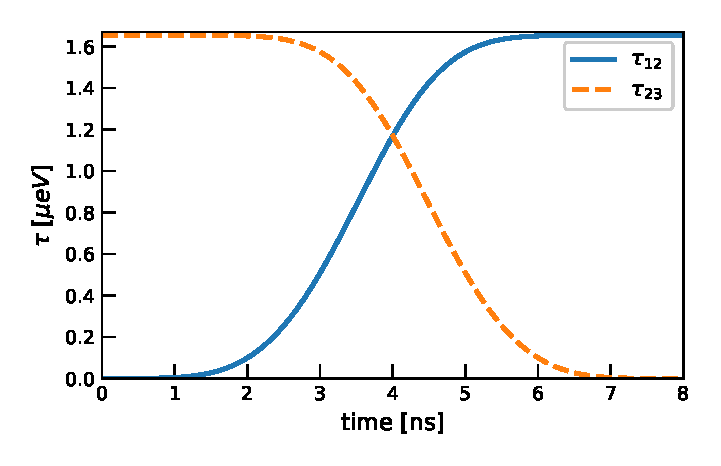
\includegraphics[width=0.7\linewidth]{STA_TQD_Pulses.eps}
	\caption{Pulses obtained for the application of the shortcuts to adiabaticity. The parameters used is $t_f=8$ ns and $\alpha_0=400\; \text{ns}^{-1}$.}
	\label{fig:STA_TQD_Pulses}
\end{figure}

In order to properly describe the system we should include SOC terms. This will give us a different population than our ansatz in Eq.~(\ref{eq:ansatz_wave_fanction}), but we will see that the difference is just the population of the state $\ket{0,\downarrow,0}$. The result is plotted in Fig~(\ref{fig:STA_TQD_Results}). The maximum population in the middle dot, summing the two possible spin configurations, is $6.6\times 10^{-4}$, which is very close to the value given by Eq.~(\ref{eq:P2_max}) of $6.8\times 10^{-4}$. We have obtained a lower population in the middle dot due to the non-vanishing probabilities $\abs{\ket{\downarrow,0,0}}^2=\abs{\ket{0,0,\downarrow}}^2\sim 10^{-4}$. Initially the hole is located at the left dot with spin up, but the same dot can be populated with opposite spin thought two possible transitions
\begin{equation}
	\begin{split}
	\ket{\uparrow,0,0}\xrightarrow{\tau}\ket{0,\uparrow,0}\xrightarrow{t_F}\ket{\downarrow,0,0}\; ,\\
	\ket{\uparrow,0,0}\xrightarrow{t_F}\ket{0,\downarrow,0}\xrightarrow{\tau}\ket{\downarrow,0,0}\; .\\
	\end{split}
\end{equation}
The fidelity obtained is very close to the unity
\begin{equation}
	1-\mathcal{F}\equiv1-\abs{\braket{\Psi(t_f)}{0,0,\uparrow}}^2\sim 10^{-9}\; .
\end{equation}
\begin{figure}[!htbp]
	\centering
	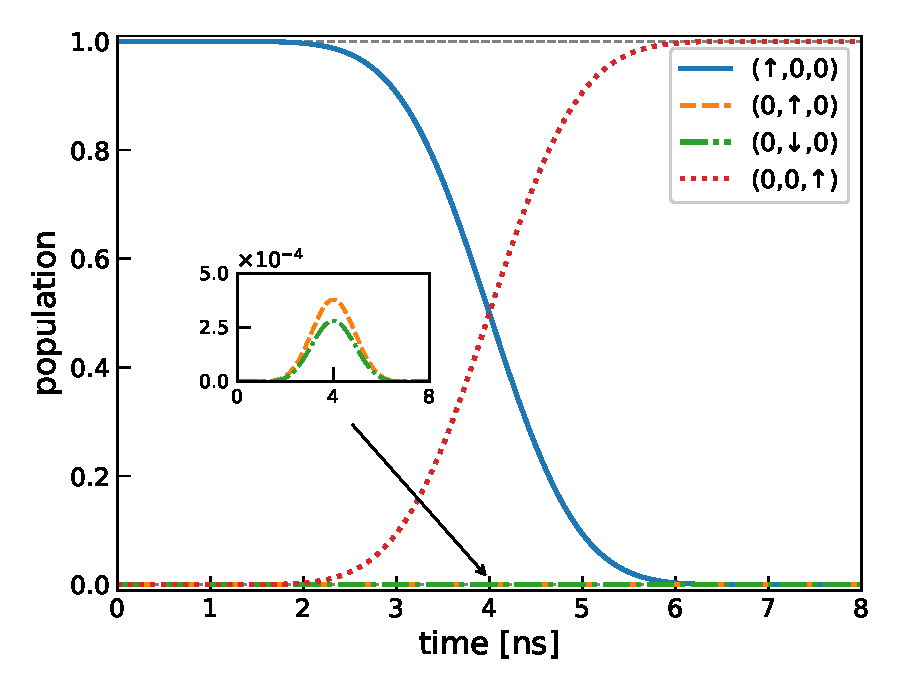
\includegraphics[width=0.8\linewidth]{STA_TQD_Results.eps}
	\caption{Result for the shortcuts to adiabaticity applied to a TQD system populated with 1 HH which has a non-negligible SOC $t_F=0.4\times\tau$. The parameter of the protocol is $\alpha_0=400$ ns. The grey dashed line denote a population equals to the unity.}
	\label{fig:STA_TQD_Results}
\end{figure}
The intensity of the pulses is controlled with the parameter $\alpha_0$, the larger it's value, the larger must be the tunnelling probability. If this parameters is lower enough we can see that the states $\ket{\downarrow,0,0}$ and $\ket{0,0,\downarrow}$ also reach a non-negligible  population Fig~(\ref{fig:STA_TQD_Results_Amplified}). In this case the population of the undesired states rises up to a value of $1\times 10^{-3}$, but the fidelity of the protocol remains constant.
\begin{figure}[!htbp]
	\centering
	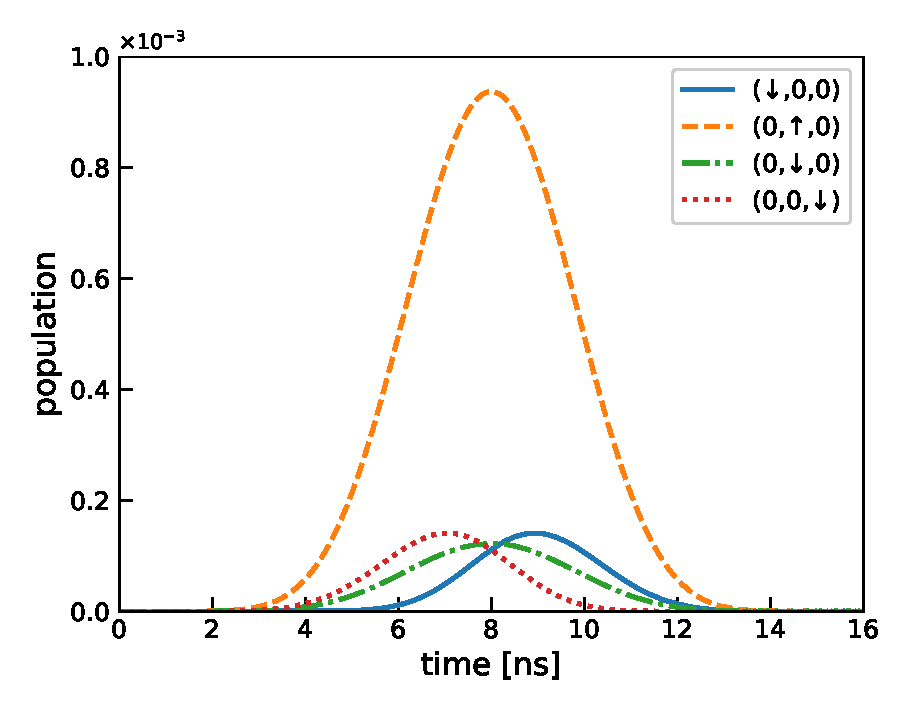
\includegraphics[width=0.7\linewidth]{STA_TQD_Results_Amplified.eps}
	\caption{Population of the non-target states in the protocol shortcuts to adiabaticity applied to a TQD system populated with 1 HH. The parameters are $\alpha_0=200$ ns and $t_f=16$ ns. Note that the initial and final states are not shown is this figure.}
	\label{fig:STA_TQD_Results_Amplified}
\end{figure}


\bibliographystyle{IEEEtran}
\bibliography{references}

\end{document}

